\documentclass[a4paper,12pt]{article}
\usepackage[utf8]{inputenc}
\usepackage[T1]{fontenc}
\usepackage[english]{babel}
\usepackage{geometry}
\usepackage{graphicx}
\usepackage{hyperref}
\usepackage{titlesec}
\usepackage{parskip}

% Configuration des marges
\geometry{hmargin=2.5cm,vmargin=2.5cm}

% Configuration des liens (Table des matières)
\hypersetup{
    colorlinks=true,
    linkcolor=black,
    filecolor=magenta,      
    urlcolor=blue,
}

\begin{document}

% --- DÉBUT DE LA PAGE DE GARDE ---
\begin{titlepage}
    % Espace vide extensible pour pousser le titre vers le bas
    \vspace*{\fill}
    
    \begin{center}
        \Huge \textbf{MACHINE LEARNING PROJECT REPORT}\\[1cm]
        \Large Prediction of the grades of students
    \end{center}
    
    % Espace vide extensible pour pousser le reste vers le bas
    \vspace*{\fill}
    
    % Alignement en bas à gauche
    \begin{flushleft}
        December 2025\\[0.5cm]
        MMN1, A4 ESILV
        \large\\
        Daphne BARAY, Sofiane BEAUMONT, Max BAUMBERGER\\[0.5cm]
    \end{flushleft}
\end{titlepage}
% --- FIN DE LA PAGE DE GARDE ---

\newpage

\tableofcontents
\newpage

\section{Introduction}

\noindent\textbf{\large Note : Ce document contient des liens hypertextes menant vers le dataset \href{https://www.kaggle.com/datasets/anassarfraz13/student-success-factors-and-insights/data }{Kaggle}, le répertoire \href{https://github.com/maxbaumberger/gradesprediction/}{GitHub} et le notebook \href{https://colab.research.google.com/drive/1d1VkLdJjlsVYWFKxfuNtNhik5k-nF-bh}{Google Colab}.}
\vspace{0.3cm}

In the modern educational landscape, understanding the factors that drive academic success is a key issue for schools and families. A student's performance is rarely the result of a single cause; instead, it comes from a complex mix of study habits, social support, and personal circumstances.

The main goal of this project is to create a predictive model to estimate a student's Exam\_Score based on these different variables. By applying Machine Learning techniques, we aim to move beyond simple observation and build a tool capable of anticipating future results. Since we are predicting a continuous numerical value, this is treated as a regression problem.

To achieve this, we used the StudentPerformanceFactors.csv dataset, that we found on \href{https://www.kaggle.com/datasets/anassarfraz13/student-success-factors-and-insights/data }{Kaggle}. This dataset contains a variety of information about the $\sim$6600 students who participated to have their data in this dataset, including their academic behaviors and social environment. Analyzing this data allows us to identify the most influential factors and propose a model that is both accurate and reliable.

This report follows the standard machine learning workflow. First, we will present a descriptive analysis and the steps taken to clean and prepare the data. Then, we will detail the modeling phase, starting with a basic Decision Tree and moving to a more advanced XGBoost model. Finally, we will compare the results to determine which approach offers the best performance.

We started by creating a \href{https://github.com/maxbaumberger/gradesprediction/}{GitHub} repository and a \href{https://colab.research.google.com/drive/1d1VkLdJjlsVYWFKxfuNtNhik5k-nF-bh}{Google Colab} notebook file to keep track and work on the project together.

\newpage
\section{Data exploration and analysis}

\subsection{Feature description}
The dataset consists of 20 variables in total, which can be categorized into numerical (quantitative) and categorical (qualitative) types.

\textbf{Numerical Variables}

These variables represent measurable quantities related to the student's performance and habits.

\begin{itemize}
    \item \textbf{Hours\_Studied (Integer):} The number of hours the student spends studying per week. This is a key indicator of academic effort.
    \item \textbf{Attendance (Integer):} The percentage of classes attended by the student. Higher attendance is often linked to better understanding of the material.
    \item \textbf{Previous\_Scores (Integer):} The scores obtained by the student in previous exams. This helps assess the student's historical academic level.
    \item \textbf{Sleep\_Hours (Integer):} The average number of hours the student sleeps per night. This reflects the student's physical well-being and rest.
    \item \textbf{Tutoring\_Sessions (Integer):} The number of tutoring sessions the student has attended per month. This indicates the level of extra academic support received.
    \item \textbf{Physical\_Activity (Integer):} The average number of hours of physical activity per week. This variable measures the student's lifestyle balance.
    \item \textbf{Exam\_Score (Integer):} Target Variable. The final score obtained by the student in the exam (0-100). This is the value we aim to predict.
\end{itemize}

\textbf{Categorical Variables}

These variables describe the student's environment, background, and personal characteristics.

\begin{itemize}
    \item \textbf{Parental\_Involvement (Object/String):} Level of parental involvement in the student's education ('Low', 'Medium', 'High').
    \item \textbf{Access\_to\_Resources (Object/String):} Availability of educational resources like internet, books, etc. ('Low', 'Medium', 'High').
    \item \textbf{Extracurricular\_Activities (Object/String):} Participation in non-academic activities ('Yes', 'No').
    \item \textbf{Motivation\_Level (Object/String):} The student's self-assessed level of motivation ('Low', 'Medium', 'High').
    \item \textbf{Internet\_Access (Object/String):} Indicates if the student has internet access at home ('Yes', 'No').
    \item \textbf{Family\_Income (Object/String):} The income level of the student's family ('Low', 'Medium', 'High').
    \item \textbf{Teacher\_Quality (Object/String):} The perceived quality of the teachers ('Low', 'Medium', 'High'). Contains missing values.
    \item \textbf{School\_Type (Object/String):} The type of school attended ('Public', 'Private').
    \item \textbf{Peer\_Influence (Object/String):} The influence of friends and peers on the student's academic life ('Positive', 'Negative', 'Neutral').
    \item \textbf{Learning\_Disabilities (Object/String):} Indicates if the student has been diagnosed with a learning disability ('Yes', 'No').
    \item \textbf{Parental\_Education\_Level (Object/String):} The highest education level attained by the parents ('High School', 'College', 'Postgraduate'). Contains missing values.
    \item \textbf{Distance\_from\_Home (Object/String):} The distance between the student's home and school ('Near', 'Moderate', 'Far'). Contains missing values.
    \item \textbf{Gender (Object/String):} The gender of the student ('Male', 'Female').
\end{itemize}

\subsection{Data Quality Assessment}
Before proceeding with the analysis, we performed a rigorous check of the dataset's quality to identify any structural errors or missing information.

\subsubsection{Data Types and Consistency}
We verified that all variables were assigned the correct data types.
\begin{itemize}
    \item Numerical variables (Hours\_Studied, Exam\_Score..) were correctly loaded as integers.
    \item Categorical variables (Parental\_Involvement, School\_Type..) were loaded as objects (strings). No immediate type conversion was required at this stage, although categorical variables will require encoding during the preprocessing phase.
\end{itemize}

\subsubsection{Missing Values Analysis}
We analyzed the dataset for null values and identified that 3 variables contained missing data :
\begin{itemize}
    \item Teacher\_Quality
    \item Parental\_Education\_Level
    \item Distance\_from\_Home
\end{itemize}
However, the proportion of missing data was very low (less than 1.36\% of the total observations). This limited amount of missing information suggests that the dataset is generally complete and reliable. Because the percentage is small, we chose to handle these values through imputation (replacing them) rather than deleting the rows, to preserve as much data as possible for training.

\begin{figure}[h]
    \centering
    % Remplacez 'image_figure1' par le nom de votre fichier image
    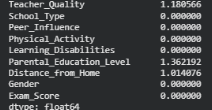
\includegraphics[width=0.6\textwidth]{image_figure1} 
    \caption{Percentage of missing values in categorial variables}
\end{figure}

\subsubsection{Duplicate Check}
We scanned the dataset for duplicate rows. The analysis confirmed that no duplicates were present (0 duplicates found), ensuring that every observation represents a unique student.

\subsection{Exploratory Data Analysis}
Once the data was validated, we conducted a visual analysis to understand the distributions and relationships between variables.

\subsubsection{Distribution of the Target Variable}
We examined the distribution of the Exam\_Score. The histogram shows that the scores follow a normal distribution (a bell-shaped curve), centered around a mean of approximately 67. This indicates that most students perform near the average, with fewer students achieving very low or very high scores. This standard distribution confirms that the target variable is well-behaved and suitable for regression models.

\begin{figure}[h]
    \centering
    % Remplacez 'image_figure2' par le nom de votre fichier image
    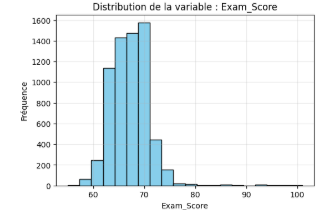
\includegraphics[width=0.6\textwidth]{image_figure2} 
    \caption{Distribution of the Exam\_Score variable}
\end{figure}

\subsubsection{Key Correlations (Numerical Variables)}
To identify the most predictive factors, we calculated the correlation between numerical variables and the Exam\_Score.
\begin{itemize}
    \item Hours\_Studied and Attendance showed the strongest positive correlations. This confirms the intuitive expectation that more study time and class presence lead to higher grades.
    \item Sleep\_Hours and Previous\_Scores also displayed positive relationships, though slightly weaker.
\end{itemize}
The correlation matrix helped us confirm that there were variables too correlated with each other that could confuse the model.

\begin{figure}[h]
    \centering
    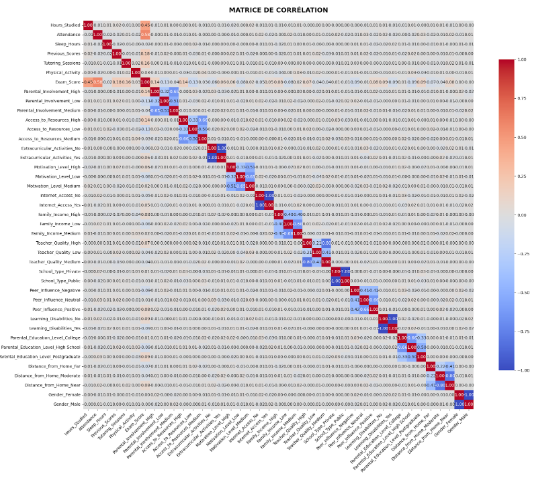
\includegraphics[width=0.8\textwidth]{image_figure3} 
    \caption{Correlation Matrix}
\end{figure}

This correlation matrix was obtained after preprocessing, and especially after encoding the categorical variables (3.2).

\subsubsection{Categorical Insights}
We analyzed how categorical variables impact performance using box plots and bar charts.
\begin{itemize}
    \item \textbf{Parental\_Involvement:} Students with "High" parental involvement tended to have higher median exam scores compared to those with "Low" involvement.
    \item \textbf{Access\_to\_Resources:} Similarly, better access to educational resources was associated with improved performance.
    \item \textbf{Motivation\_Level:} Contrary to what we could think, there is no clear trend where higher self-reported motivation correlates with better results.
\end{itemize}

\begin{figure}[h]
    \centering
    % Remplacez 'image_figure4' par le nom de votre fichier image
    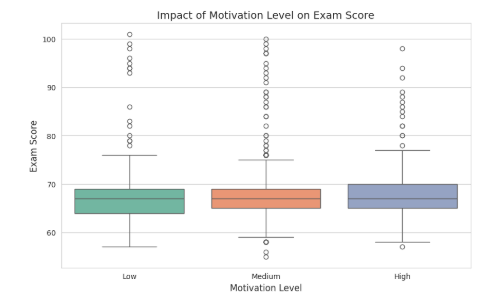
\includegraphics[width=0.8\textwidth]{image_figure4} 
    \caption{Boxplots of the exam scores in function of the different motivation levels}
\end{figure}

This exploration highlights that student performance is driven by a combination of personal habits (study, sleep) and environmental support (parents, resources). These insights guided our feature selection for the machine learning models.

\section{Preprocessing}
Before feeding the data into machine learning models, we applied a series of transformations to ensure the dataset was clean, numerical, and optimized for learning.

\subsection{Feature Selection}
To improve model efficiency and reduce noise, we performed feature selection based on correlation. We calculated the correlation of each new variable with the target (Exam\_Score). We decided to keep only the variables that showed a correlation coefficient of at least 0.1 (absolute value). This ensures the model focuses only on the most relevant factors, reducing complexity and the risk of overfitting. As a result, variables with very weak relationships to the target were removed.

\begin{figure}[h]
    \centering
    % Remplacez 'image_figure5' par le nom de votre fichier image
    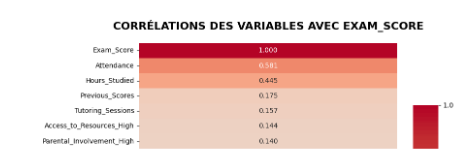
\includegraphics[width=0.8\textwidth]{image_figure5} 
    \caption{Correlation Variables with Exam\_Score}
\end{figure}

\subsection{Encoding Categorical Variables}
Machine learning algorithms require numerical input. Since our dataset contained many categorical variables (like Parental\_Involvement or School\_Type), we transformed them using One-Hot Encoding. This process converts each category into a new binary column (0 or 1). For example, a "Gender" column is split into "Gender\_Male" and "Gender\_Female". This resulted in an expanded dataset where all features were numeric.

\subsection{Handling Missing Values}
As identified in the data quality assessment, three categorical variables (Teacher\_Quality, Parental\_Education\_Level, Distance\_from\_Home) contained a small number of missing values. To address this, we used Mode Imputation. We replaced the missing entries with the most frequent category of each respective column. This method allows us to retain all observations without introducing artificial noise.

\subsection{Feature Scaling}
After filtering the variables, we applied Standard Scaling (StandardScaler) to the entire feature set (X). This transformation standardizes the data so that each variable has a mean of 0 and a standard deviation of 1. Scaling is crucial because it prevents variables with large ranges (like Hours\_Studied) from dominating variables with smaller ranges during the training process.

\subsection{Train/Test Split}
Finally, we split the processed dataset into two distinct subset: a training set containing 70\% of our data, used to train the models, and a test set with the rest (30\%) that’s kept separate and used only to evaluate the final performance.
We used a fixed random\_state=42 to ensure the split is reproducible.

\section{Machine Learning Models and Optimization}
We implemented a progressive modeling strategy by testing three distinct approaches to maximize predictive accuracy, starting with a simple Decision Tree and advancing to an ensemble Bagging model and finally an optimized XGBoost algorithm.

\subsection{Baseline Model: Decision Tree}
We began our analysis with a Decision Tree Regressor as our baseline model because it is intuitive and easy to interpret. The initial unoptimized tree showed signs of overfitting, meaning it learned the training data too specifically and struggled to generalize to new students. To address this, we used GridSearchCV to systematically test various combinations of hyperparameters such as the maximum depth of the tree and the minimum samples required to split a node. The best configuration found by the search significantly reduced the variance of the model, providing a much more stable and reliable baseline for further comparison.

\subsection{Ensemble Method: Bagging}
Building on the optimized Decision Tree, we implemented a Bagging Regressor to further improve performance. This method creates multiple versions of the same model (in this case, 100 optimized trees) trained on random subsets of the data and then averages their predictions. This approach proved effective because averaging the results of many trees generally reduces the risk of errors and makes the model more robust to outliers in the student data compared to a single tree.

\subsection{Advanced Model: XGBoost}
Finally, we tested XGBoost (Extreme Gradient Boosting), a state-of-the-art algorithm known for its high performance in regression tasks. Unlike Bagging, which builds trees in parallel, Boosting builds them sequentially so that each new tree attempts to correct the errors of the previous one. Given the complexity of this algorithm, we used RandomizedSearchCV to efficiently find the best hyperparameters by testing 40 different combinations of settings like learning rate, number of estimators, and tree depth. The search identified an optimal configuration that provided the highest accuracy of all the models we evaluated.

\subsection{Hyperparameter Tuning Strategy}
As said, to ensure our models performed at their best potential, we did not rely on default settings. Instead, we implemented a rigorous optimization phase to identify the most effective hyperparameters for each algorithm.

\subsubsection{Grid Search for Decision Tree}
For the Decision Tree model, we employed GridSearchCV (Grid Search with Cross-Validation). Since the number of parameters to tune was relatively small, we could afford to test every possible combination in our defined search space. We systematically varied the max\_depth to control complexity, along with min\_samples\_split and min\_samples\_leaf to prevent the tree from growing too specific to the training data. We used 5-fold Cross-Validation, meaning the model was trained and validated 5 times on different subsets of data for each combination, ensuring the results were reliable and not due to chance.

\subsubsection{Randomized Search for XGBoost}
For the XGBoost model, the search space was significantly larger and more complex. Testing every combination would have been computationally too expensive. Therefore, we adopted RandomizedSearchCV. Instead of checking every point, this method randomly sampled 40 different configurations from a specified distribution of hyperparameters. We adjusted boosting parameters, such as learning\_rate (how fast the model learns), n\_estimators (number of trees), and max\_depth. We used 3-fold Cross-Validation to evaluate each of the 40 iterations. This approach allowed us to explore a wide range of possibilities efficiently and find a high-performing configuration without excessive calculation time.

\subsubsection{Optimization Metric}
For both strategies, we optimized the models to minimize the MSE. This ensures that the selected models are those that make the smallest average errors in their predictions.

\begin{figure}[h]
    \centering
    % Remplacez 'image_figure6' par le nom de votre fichier image
    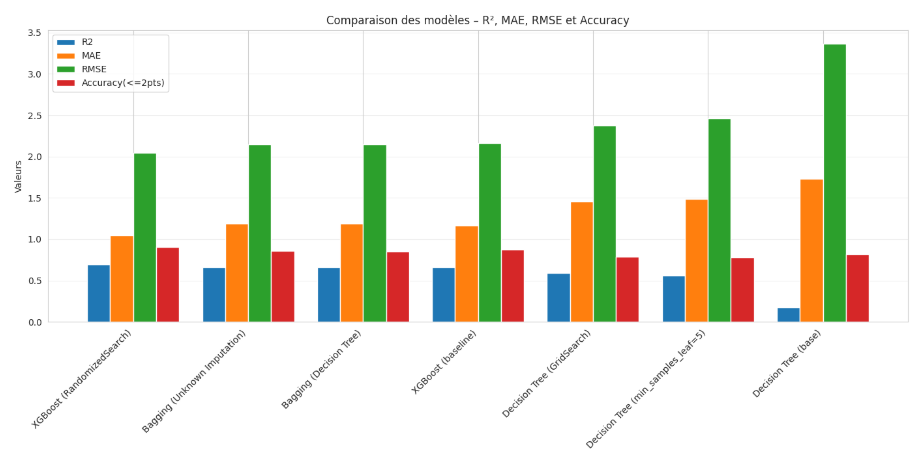
\includegraphics[width=0.9\textwidth]{image_figure6} 
    \caption{Comparison of the models we tested}
\end{figure}

\section{Analysis of Results}
After training and optimizing our three candidate models, we compiled their performance metrics to identify the most effective solution.
The results reveal a clear hierarchy in model performance:
\begin{itemize}
    \item Decision Tree (Baseline) showed the lowest predictive power with an R² of roughly 0.59 (optimized). While interpretable, it struggled to capture the complex, non-linear relationships between student habits and exam scores.
    \item Bagging Regressor significantly improved upon the single tree, reaching an R² of 0.666. By averaging 100 trees, it successfully reduced variance and smoothed out errors.
    \item XGBoost emerged as the best performing model with an R² of 0.70 and the lowest Root Mean Squared Error (RMSE $\approx$ 2.03).
\end{itemize}
The superiority of XGBoost can be attributed to its boosting mechanism. Unlike Bagging, which builds trees independently, XGBoost learns sequentially. It specifically targeted the "hard-to-predict" students where previous trees had failed, iteratively correcting errors. This allowed it to fine-tune its predictions more effectively than the other models.

The final MAE of 1.04 for the XGBoost model is particularly encouraging. In practical terms, this means that on average, our model's prediction is only 1 point away from a student's actual exam score (on a scale of 0-100). For an educational tool intended to flag students at risk or estimate performance, this level of precision is highly reliable.

\subsubsection{Error Analysis by Actual Score}

To critically assess the model's reliability across the entire score range, we conducted a detailed error analysis, defining a prediction as "correct" if the absolute error was  ≤ 2 points.
The analysis showed that precision is directly proportional to score frequency:
Best Performance: Accuracy is highest 95 % for scores around the mean (66-74), where the training data is dense.
Highest Errors: The largest errors are systematically found on rare, extreme scores (both high and low). This confirms the model tends to generalize where training data is rare ( scores 98, 87, which had 0% accuracy).
This indicates the model is highly robust for the average student but less reliable for predicting highly exceptional or extremely low performance.


\begin{figure}[h]
    \centering
    % Remplacez 'image_figure7' par le nom de votre fichier image
    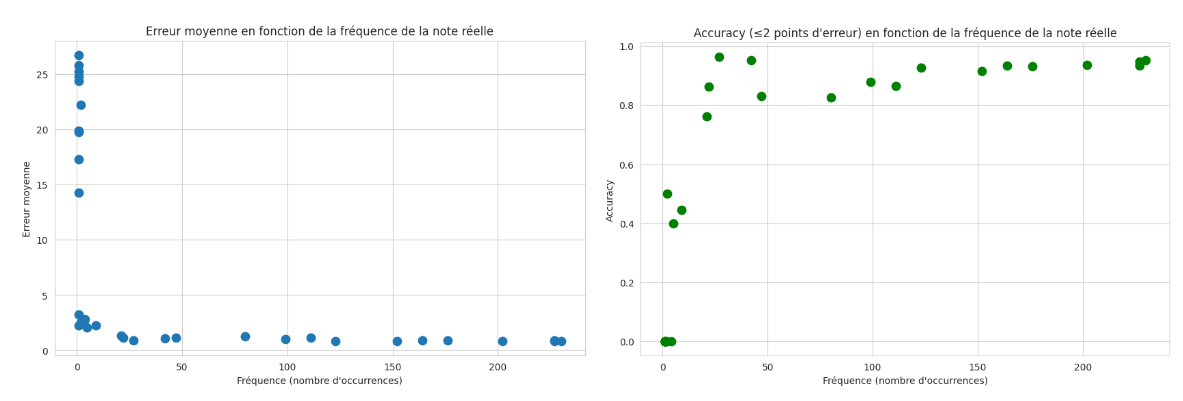
\includegraphics[width=0.8\textwidth]{image_figure7} 
    \caption{Average error and Accuracy as a function of frequency}
\end{figure}

\section{Conclusion}
This project aimed to predict student exam scores using machine learning techniques based on various demographic, social, and academic factors. By analyzing the StudentPerformanceFactors.csv dataset, we successfully built and optimized several predictive models to address this regression problem.

Our exploratory analysis and modeling confirmed that student success is largely driven by measurable behaviors. Academic habits such as attendance and weekly study hours emerged as the strongest predictors of performance, whereas background factors like teacher quality or distance from home had a negligible impact. In terms of modeling, we observed a clear progression in accuracy. The baseline Decision Tree was too simple to capture the full complexity of the data, resulting in an R² of approximately 0.59. The introduction of the Bagging Regressor improved robustness by averaging predictions, raising the score to 0.66. Ultimately, the XGBoost algorithm proved to be the most effective solution, achieving an R² of roughly 0.70 and a low Mean Absolute Error of about 1 point. This level of precision confirms that the model is reliable enough to be used as a diagnostic tool to identify students at risk.

\end{document}